\graphicspath{{chapt_dutch/}{intro/}{chapt2/}{chapt3/}{chapt4/}{chapt5/}{chapt6/}{chapt7/}{chapt8/}}
%\usepackage{zref-xr}

% Header
\renewcommand\evenpagerightmark{{\scshape\small Chapter 3}}
\renewcommand\oddpageleftmark{{\scshape\small LHC and the CMS Experiment}}

\renewcommand{\bibname}{References}

\hyphenation{}

\chapter[LHC and the CMS Experiment]%
{LHC and the CMS detector}
\label{chap:2}

\section{The Large Hadron Collider at CERN}
\label{sec:lhc}
The Large Hadron Collider (LHC) is a circular protons and heavy ions collider with a circumference of ~27 km, 100 m underground, operated at the laboratories of the European Organization for Nuclear Research (CERN\footnote{Called Conseil Européen pour la Recherche Nucléaire.}) in Geneva, Switzerland \cite{Bruning:lhc}. LHC has designed to operate at centre of mass (CoM) energy $\sqrt{s}$ = 14 TeV which makes it the world's most powerful accelerator. Proton-proton (pp) collision is the main part of the LHC physics program where part of the machine schedule is periodically dedicated to the delivery of heavy-ion collisions. The accelerator complex at CERN is a succession of machines to accelerate particles beams in many steps before injecting into the main ring. Protons are first accelerated in different linear accelerators (LINAC) to the energy of 50 MeV. The beam is then injected into the Proton Synchrotron Booster (PSB) followed by the Proton Synchrotron (PS), which pushes the beam to 25 GeV. Protons are then sent to the Super Proton Synchrotron (SPS) where they are accelerated to 450 GeV. Most of the pre-accelerators in the chain have their own experimental halls where beams are used for different purposes such as other particle-physics experiments, test beams or irradiation of detector material for radiation-hardness studies.\\
The protons beams are finally transferred to the largest ring of the LHC to attain 6.5 TeV energy per beam. It includes two adjacent beam pipes, each containing one of two colliding beams, which travel in opposite directions in the collider ring. Ultrahigh beam vacuum ($10^{10}$ Torr) is created to avoid possible collision with gas molecules. The beams are guided and focused in circular trajectory by using superconducting (1.9-4 K) dipole and quadrupole magnets. In the LHC, beams are accelerated/decelerated by the electromagnetic field generated by radio-frequency (RF) cavities (eight per beam) located along the collider ring: each of these cavities also operates in superconducting state, at a temperature of approximately 4.5 K, and can deliver a voltage of 2 MV at a frequency of 400 MHz. The main role of the RF cavities is to keep the 2808 proton bunches tightly bunched to ensure high luminosity at the collision points and hence maximize the number of collisions (luminosity). The two beams are crossing each other at four interaction points where detectors installed. The CERN accelerator complex with four interaction points is shown in Fig.\ref{fig:LHC_complex}.\\

\begin{figure}[h]
\centering
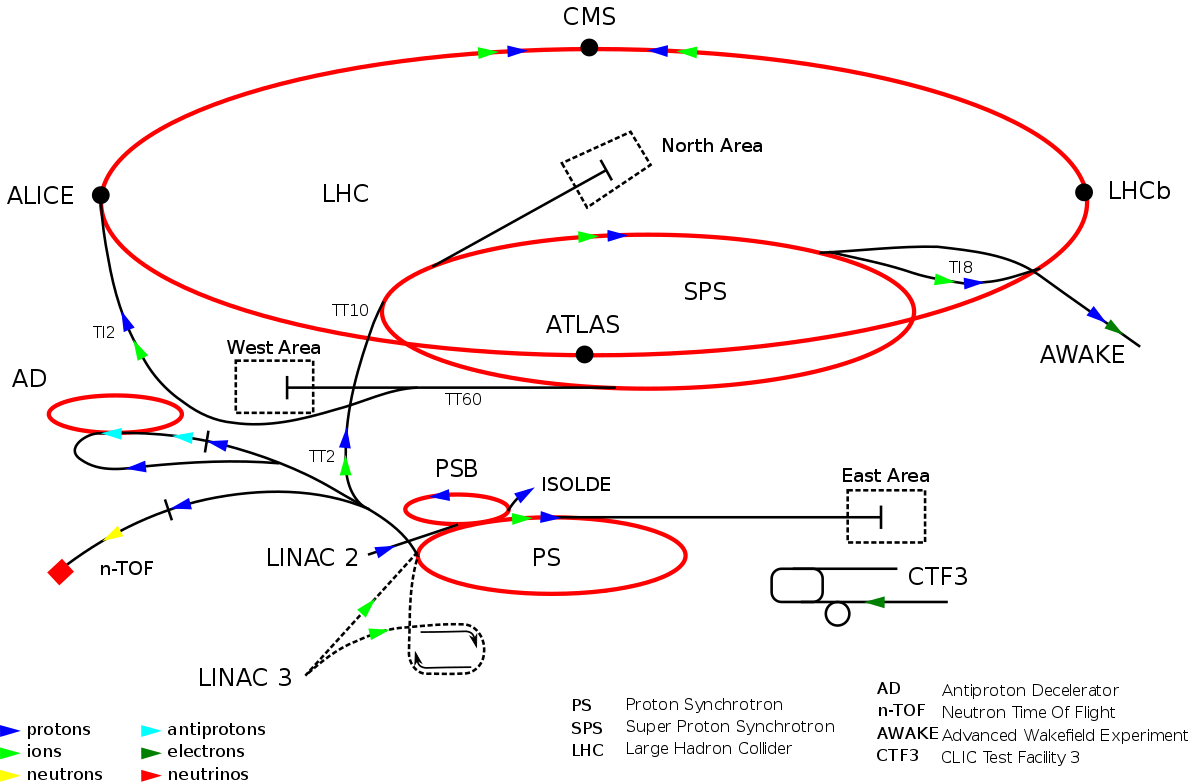
\includegraphics[width=0.9\textwidth]{fig/chapt3/LHC_complex.png}
\caption{\label{fig:LHC_complex} The CERN accelerator complex. The proton injection chain for the LHC
starts from the LINAC2 and proceeds through the Booster, PS and SPS.}
\end{figure}

The performance of an accelerator is measured in terms of instantaneous luminosity $\mathcal{L}$, the most important characteristic of a collider is, that ties event rate to the cross-section ($\sigma$) of a process:
\begin{equation}
\frac{dN_{i}}{dt} = \sigma_{i} \mathcal{L}(t)
\end{equation}
Where i indicates any general process and $\mathcal{L}(t)$ is the instantaneous luminosity that depends on the number of interaction per unit time. The machine instantaneous luminosity related to the beam parameters, and can be written as:
\begin{equation}
\mathcal{L} = \frac{f_{rel}N_{b}^{2}n_{b}\gamma_{r}}{4\pi\epsilon_{n}\beta^{\ast}}F
\end{equation}
where $f_{rev}$ = 11 kHz is the revolution frequency, $N_{b}$ is the number of particles per bunch, $n_{b}$ is the number of bunches per beam, $\epsilon_{n}$ is the normalized transverse beam emittance, $\beta^{\ast}$ is the beta function at the collision point, which measures the beam focalization and is corrected by the relativistic gamma factor $\gamma_{r}$, and F is a geometric luminosity reduction factor that accounts for the crossing angle at the interaction point \cite{lumi_formula}. The amount of data delivered by a collider is measured in terms of total integrated luminosity $L = \int\mathcal{L}dt$ and measured in unit fb$^{-1}$. Since discoveries in particle physics depends on statistics, the higher luminosity, the more chances physicists have to discover a particle or process.\\
During 2016, the LHC has operated at CoM energy $\sqrt{s} = 13$ TeV with a bunch spacing of 25 ns. Reducing the $\beta^{\ast}$ parameter from 80 cm to 40 cm, the the nominal LHC luminosity crossed the record value $10^{34}$ cm$^{-2}$ s$^{-1}$ in late summer 2016. The instantaneous luminosity delivered by LHC (blue) and recorded by CMS (yellow) is shown in \ref{fig:cms_lumi}(a) and the total integrated luminosity is in \ref{fig:cms_lumi}(b) during 2016.   


\begin{figure}[htp]
\centering
\begin{tabular}{cc}
\hspace{-0.3cm}
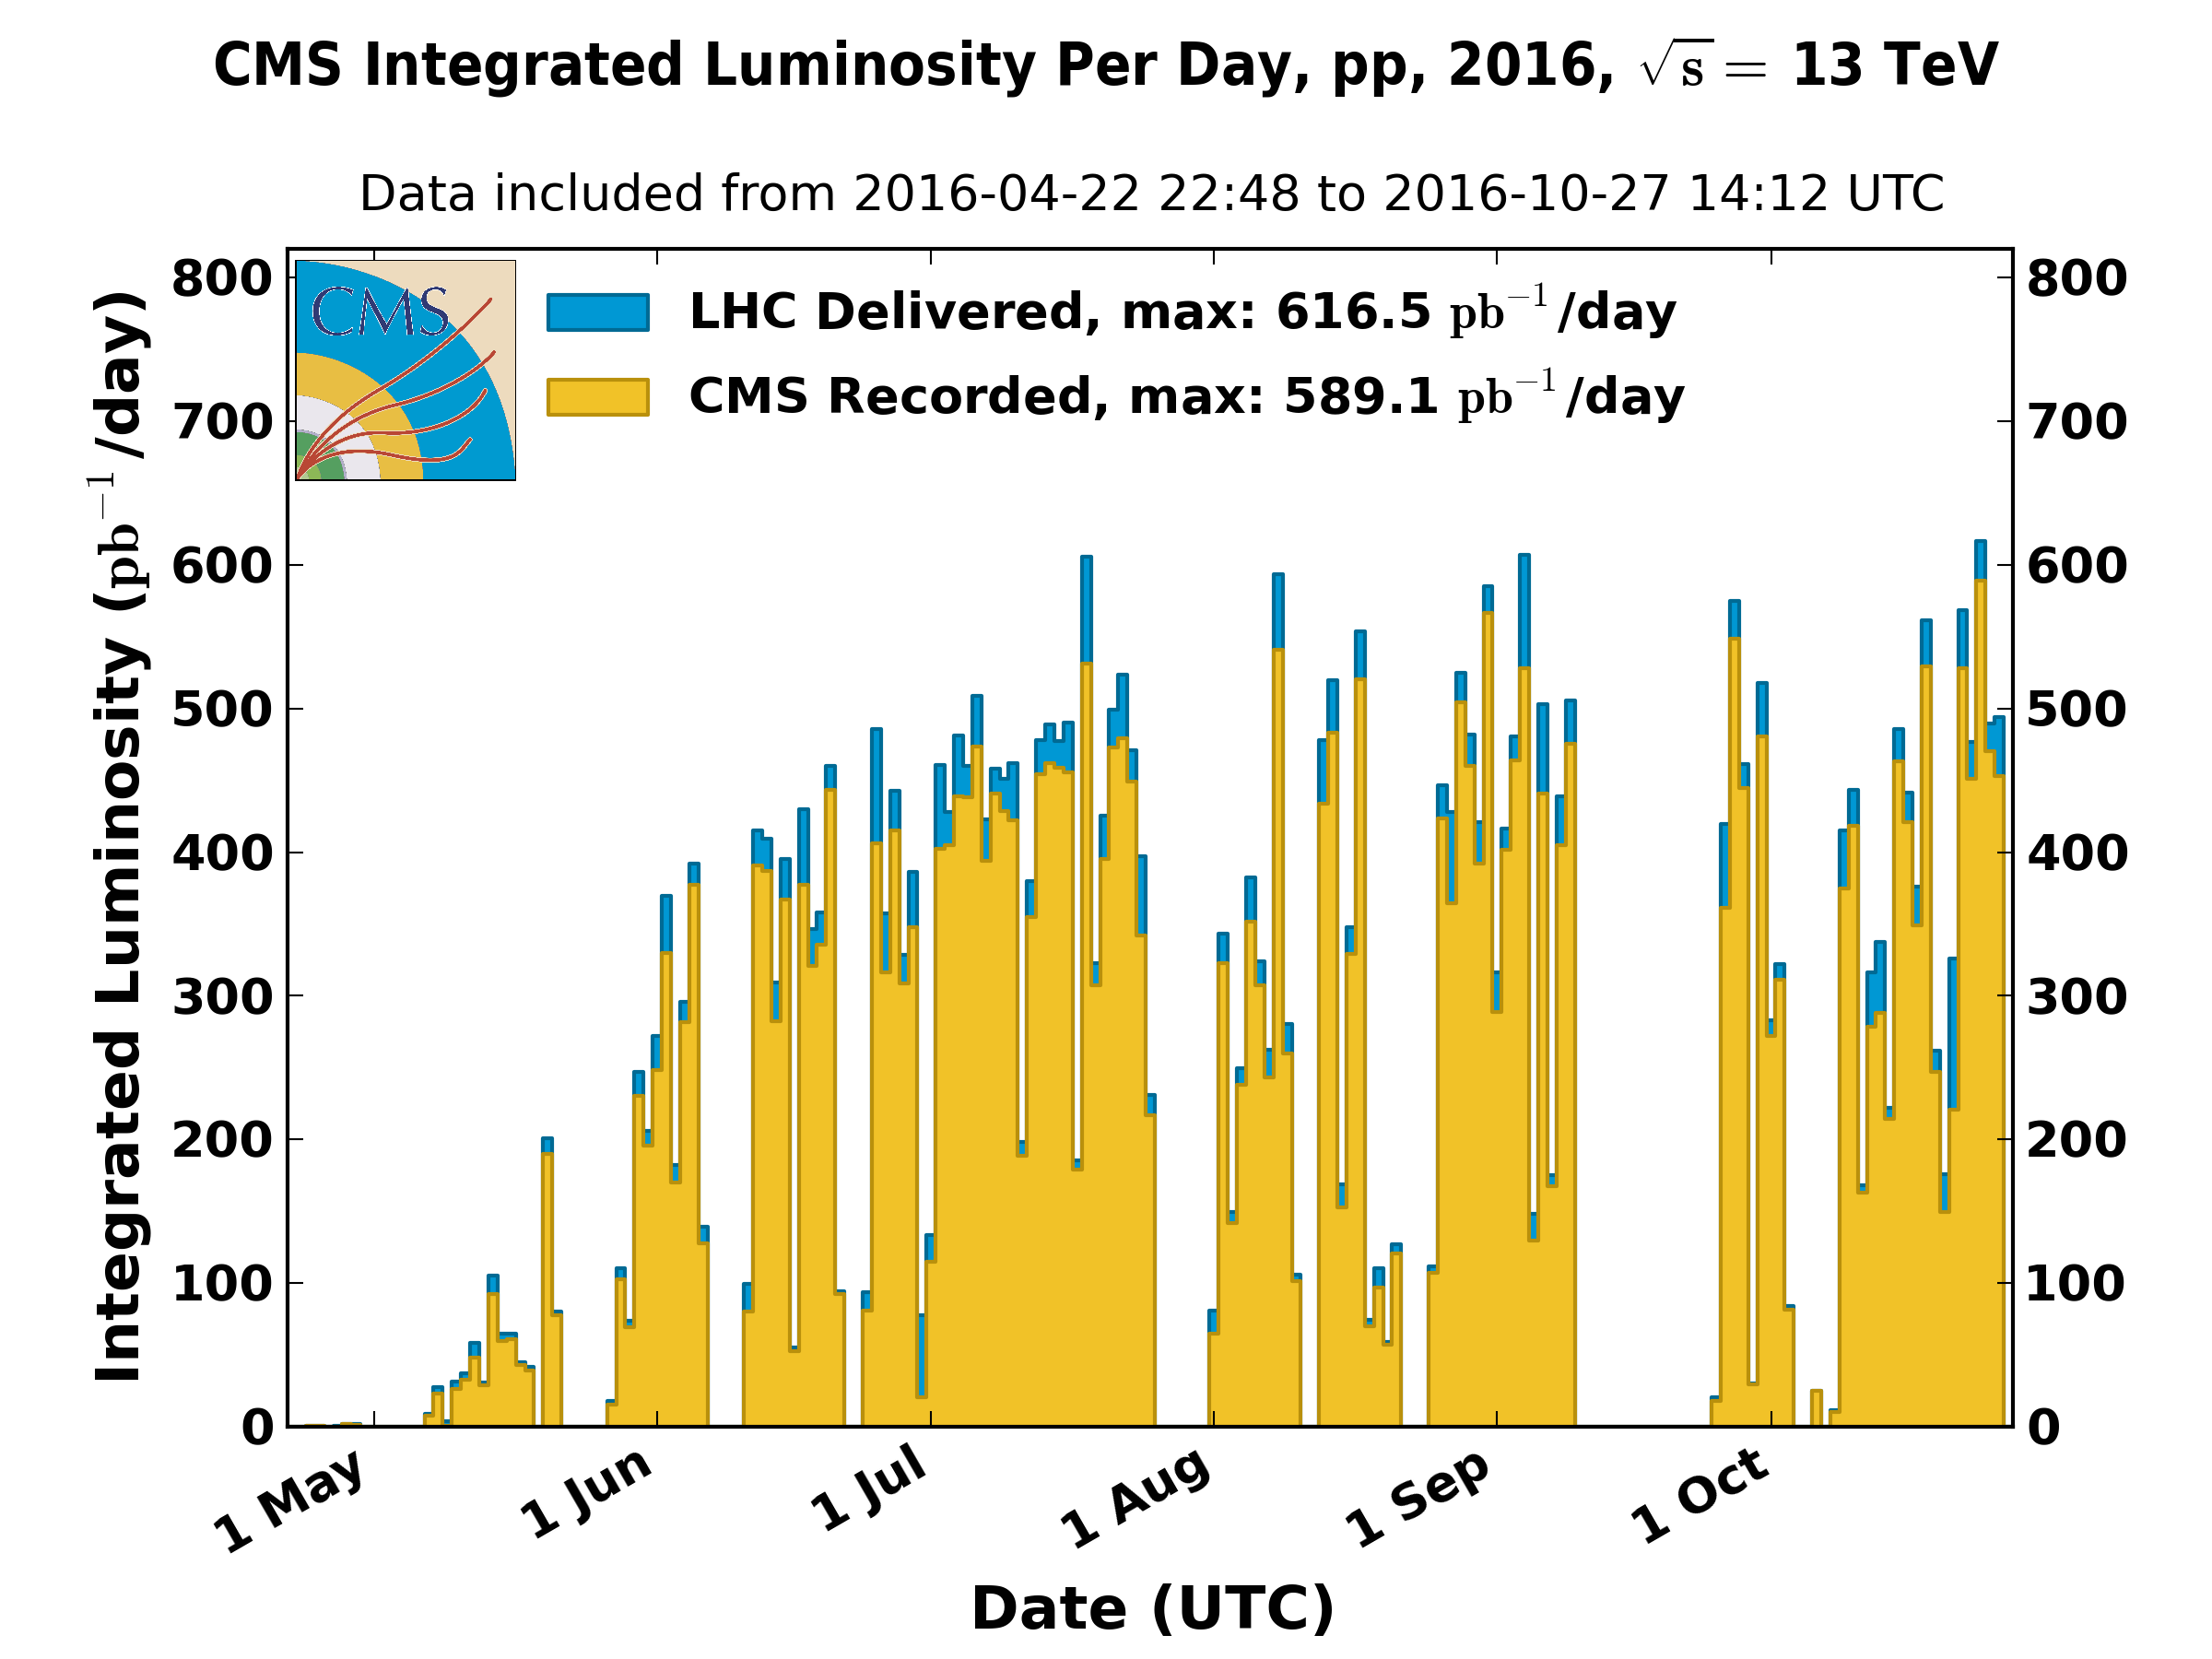
\includegraphics[scale=0.39]{fig/chapt3/int_lumi_per_day_pp_2016.png}
& \hspace{-0.5cm} 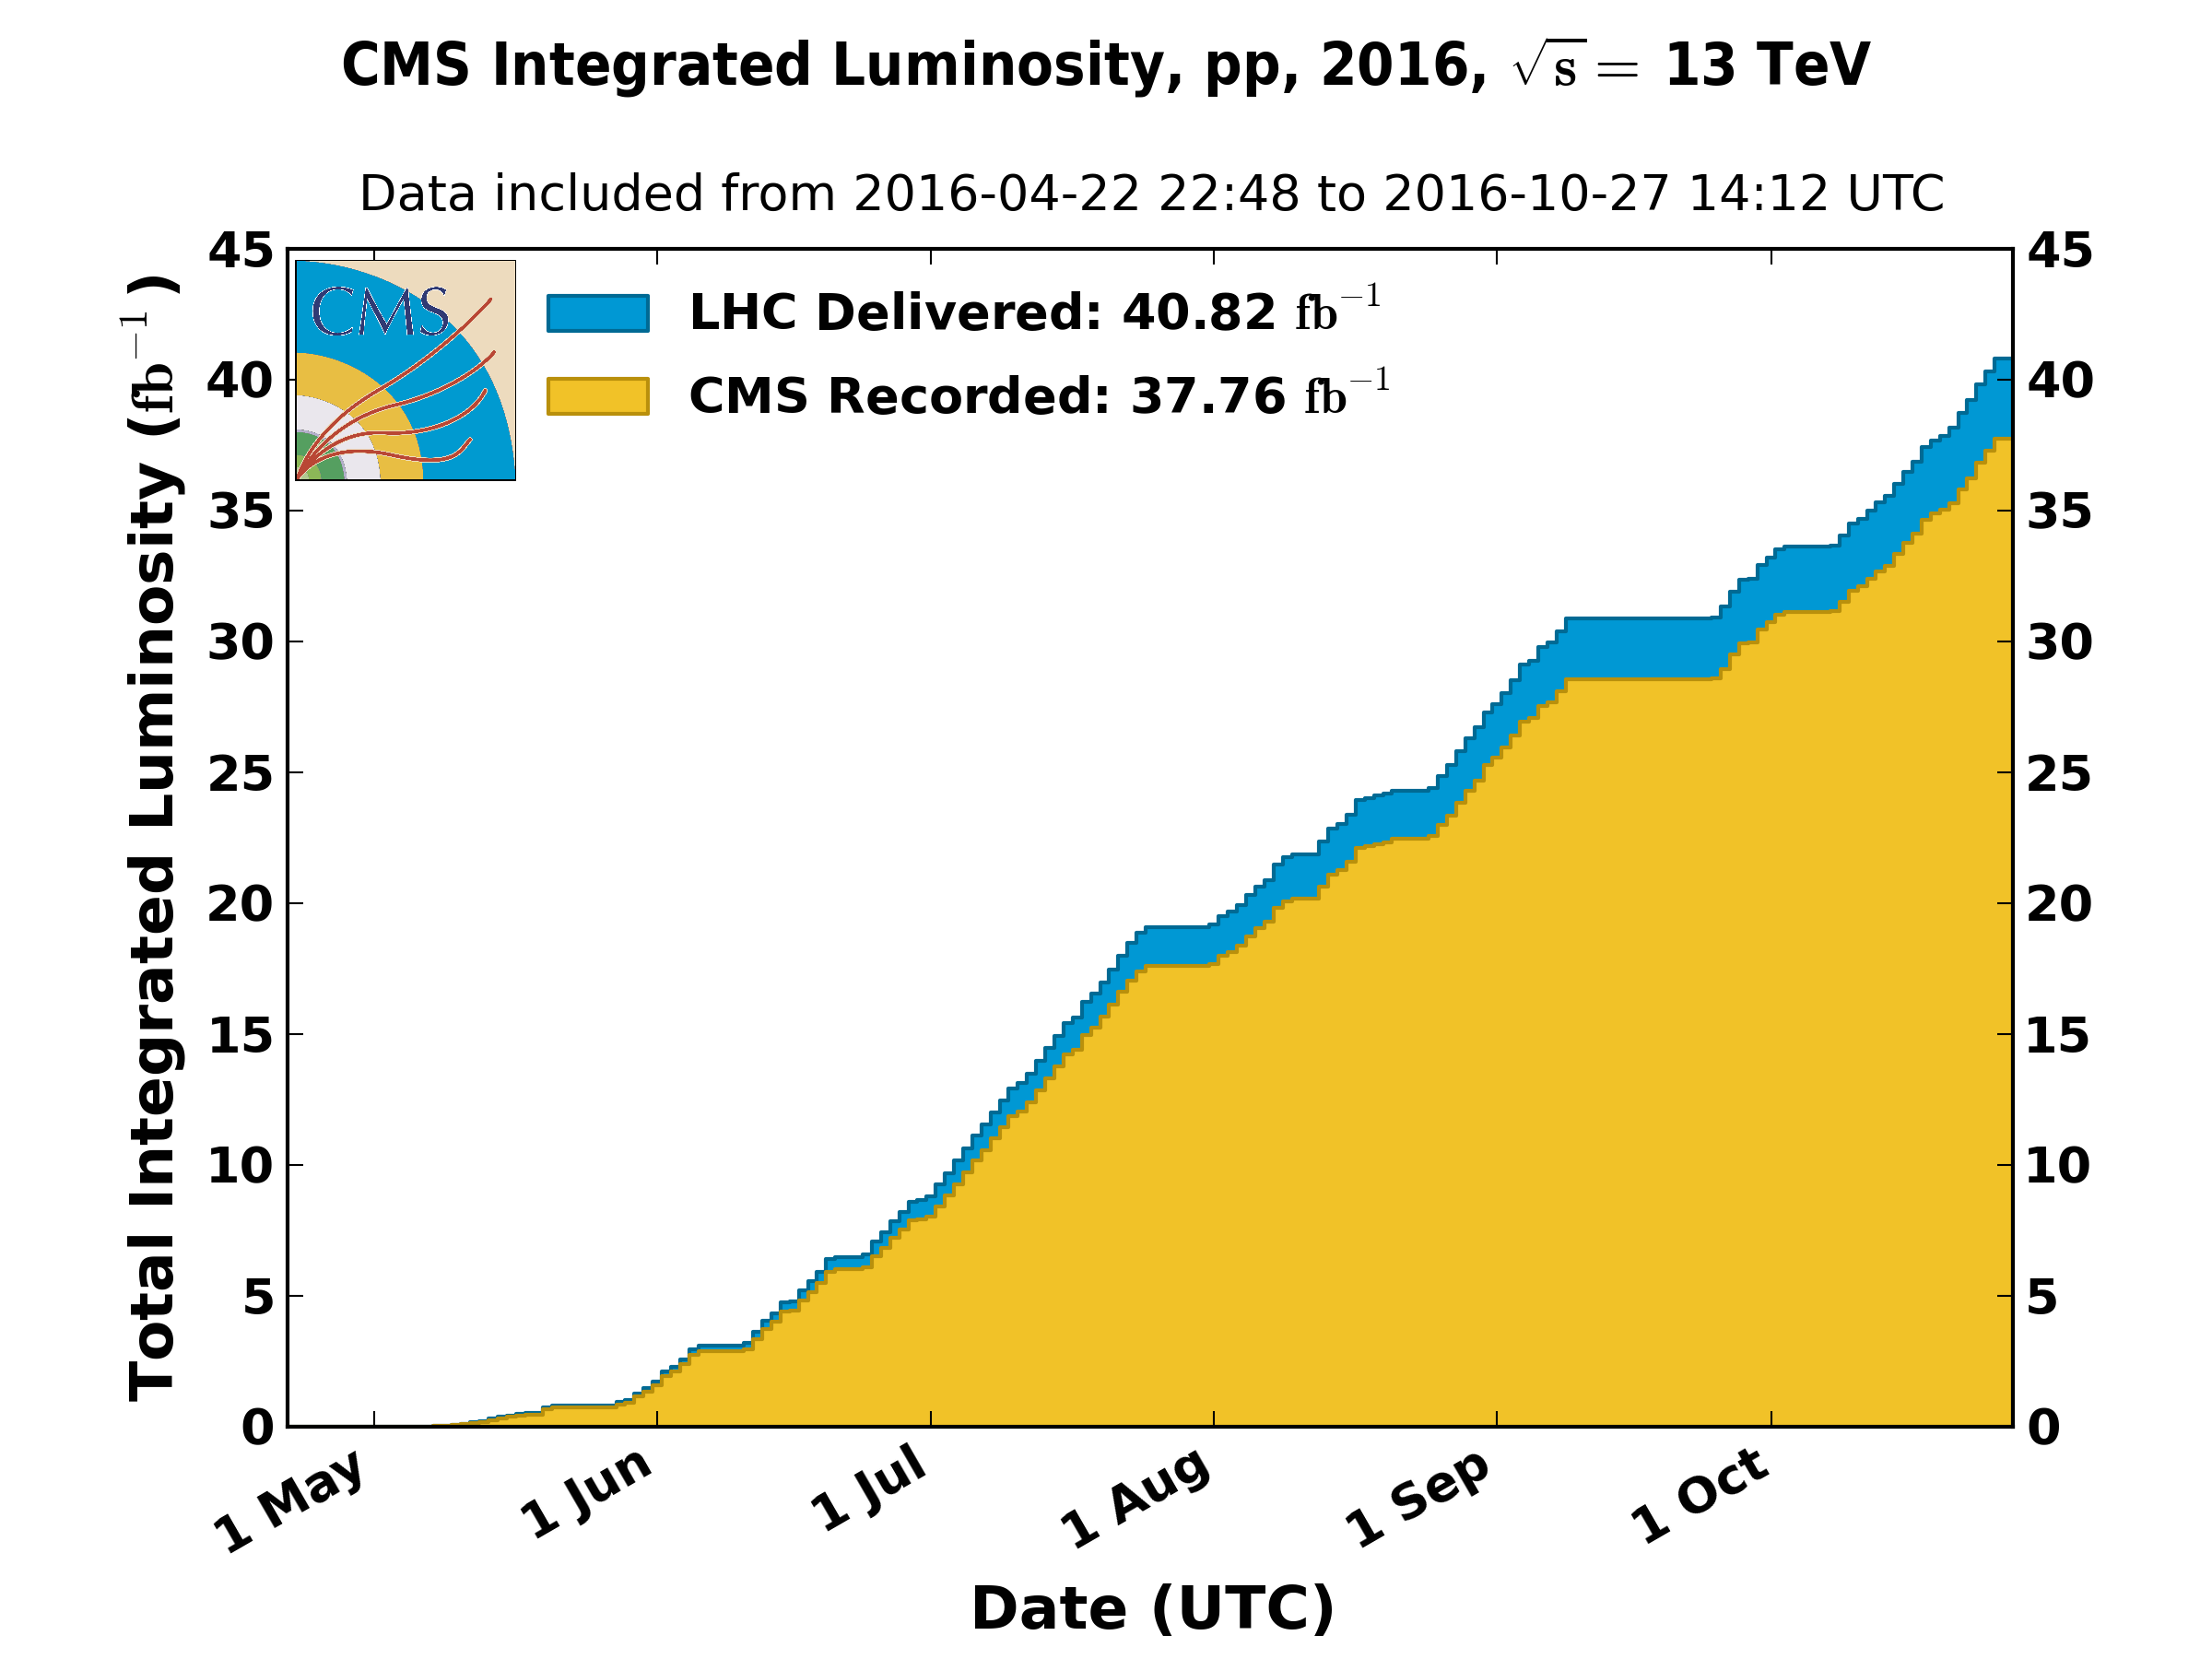
\includegraphics[scale=0.39]{fig/chapt3/int_lumi_per_day_cumulative_pp_2016.png}\\
   ($\mathbf{a}$)\qquad&($\mathbf{b}$)\qquad\\
\end{tabular}
\caption{The evolution of the instantaneous luminosity per day (a) and the integrated luminosity (b) delivered by the LHC (blue) and recorded by CMS (yellow) in 2016. The plots are taken from online cmstwiki \cite{twiki:cms_lumi}.}\label{fig:cms_lumi}
\end{figure}

Among the four detectors, two of them ATLAS (A Toroidal LHC ApparatuS) and CMS (Compact Muon Solenoid) are the largest and multi-purpose experiments. Their main focus is on the precise measurements of the SM as well as searches of BSM physics. ALICE (A Large Ion Collider
Experiment) is designed for heavy-ion collisions to study the physics of strongly interacting matter at extreme energy densities; and to study the quark-gluon plasma. Hadron Collider beauty (LHCb) experiment is designed to study the heavy flavour beauty hadron physics.

\section{The CMS Experiment at LHC}\label{sec:cms}
The CMS \cite{cms_exp} is one of the two multi-purpose experiments installed at the LHC cavern with a design to study a wide range particle and heavy ion physics measurements. Its primary goals are to elucidate the nature of the electroweak symmetry breaking mechanism linked to the Higgs mechanism, the search for physics Beyond the Standard Model (BSM) and the precise measurements of SM processes. An overview of the whole detector is shown in Fig. \ref{fig:CMS_exper}. The general concept driving the detector design is the configuration of the magnetic field needed to bend the trajectory of the charged particles, especially muons, to have good resolution in measuring high momentum. The CMS detector has a superconducting solenoid magnetic, producing a field of 3.8 T parallel to the beam axis, encapsulates a high-quality tracking system and calorimeters. The muon system is installed outside the magnet in 4 stations and interleaved with return yoke. The magnetic field is strong enough to saturate 1.5 m of iron. Each muon station consists of several layers of aluminium drift tubes (DT) in the barrel region (coaxial to the beam axis) and cathode strip chambers (CSCs) in the endcap region (perpendicular to the beam axis), complemented by resistive plate chambers (RPCs). The CMS detector is relatively compact in spite of its heavy weight, 12,500 Tons, (compare to ATLAS) with a length of 21.6 m and a diameter of 14.6 m. \\
\begin{figure}[h!]
%\centering
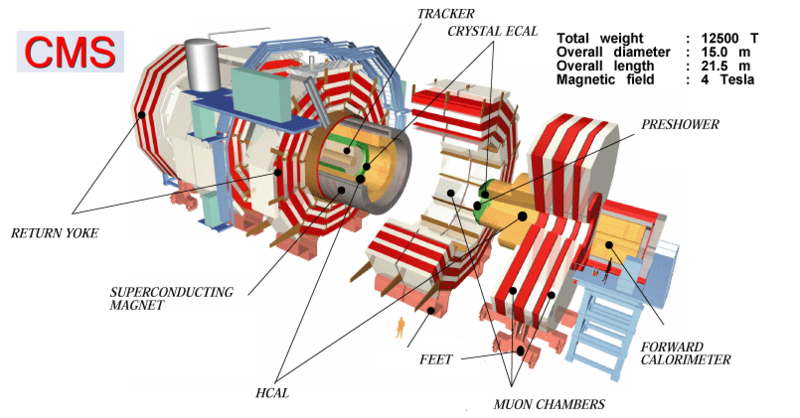
\includegraphics[width=1.05\textwidth]{fig/chapt3/CMS_exper.png}
%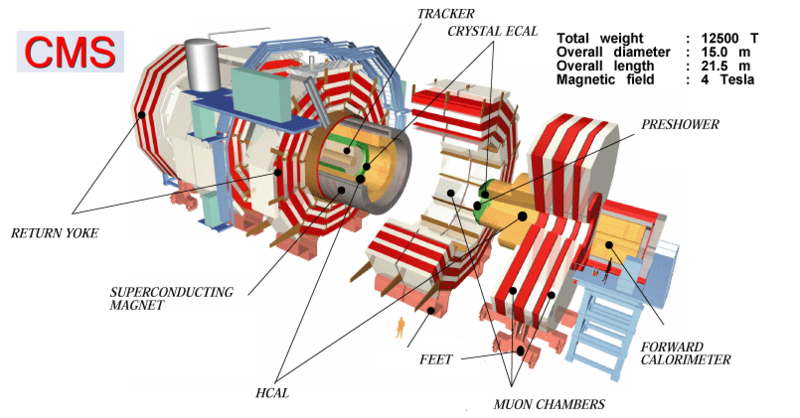
\includegraphics[scale=0.4, trim=20 50 60 30,clip]{fig/chapt3/CMS_exper.png}
\caption{\label{fig:CMS_exper} An overview of the CMS detector showing the major sub detectors.}
\end{figure}
The CMS experiment adopted a cylindrical coordinate system with its origin at the nominal interaction point in the center of the detector.    The direction of the z-axis is chosen along the anti-clockwise beam and it is referred as longitudinal. The x-axis points radially towards the center of the LHC ring and the y-axis is vertical and pointing upwards shown in Fig.\ref{fig:CMS_coordinates}. 
\begin{figure}[h!]
\centering
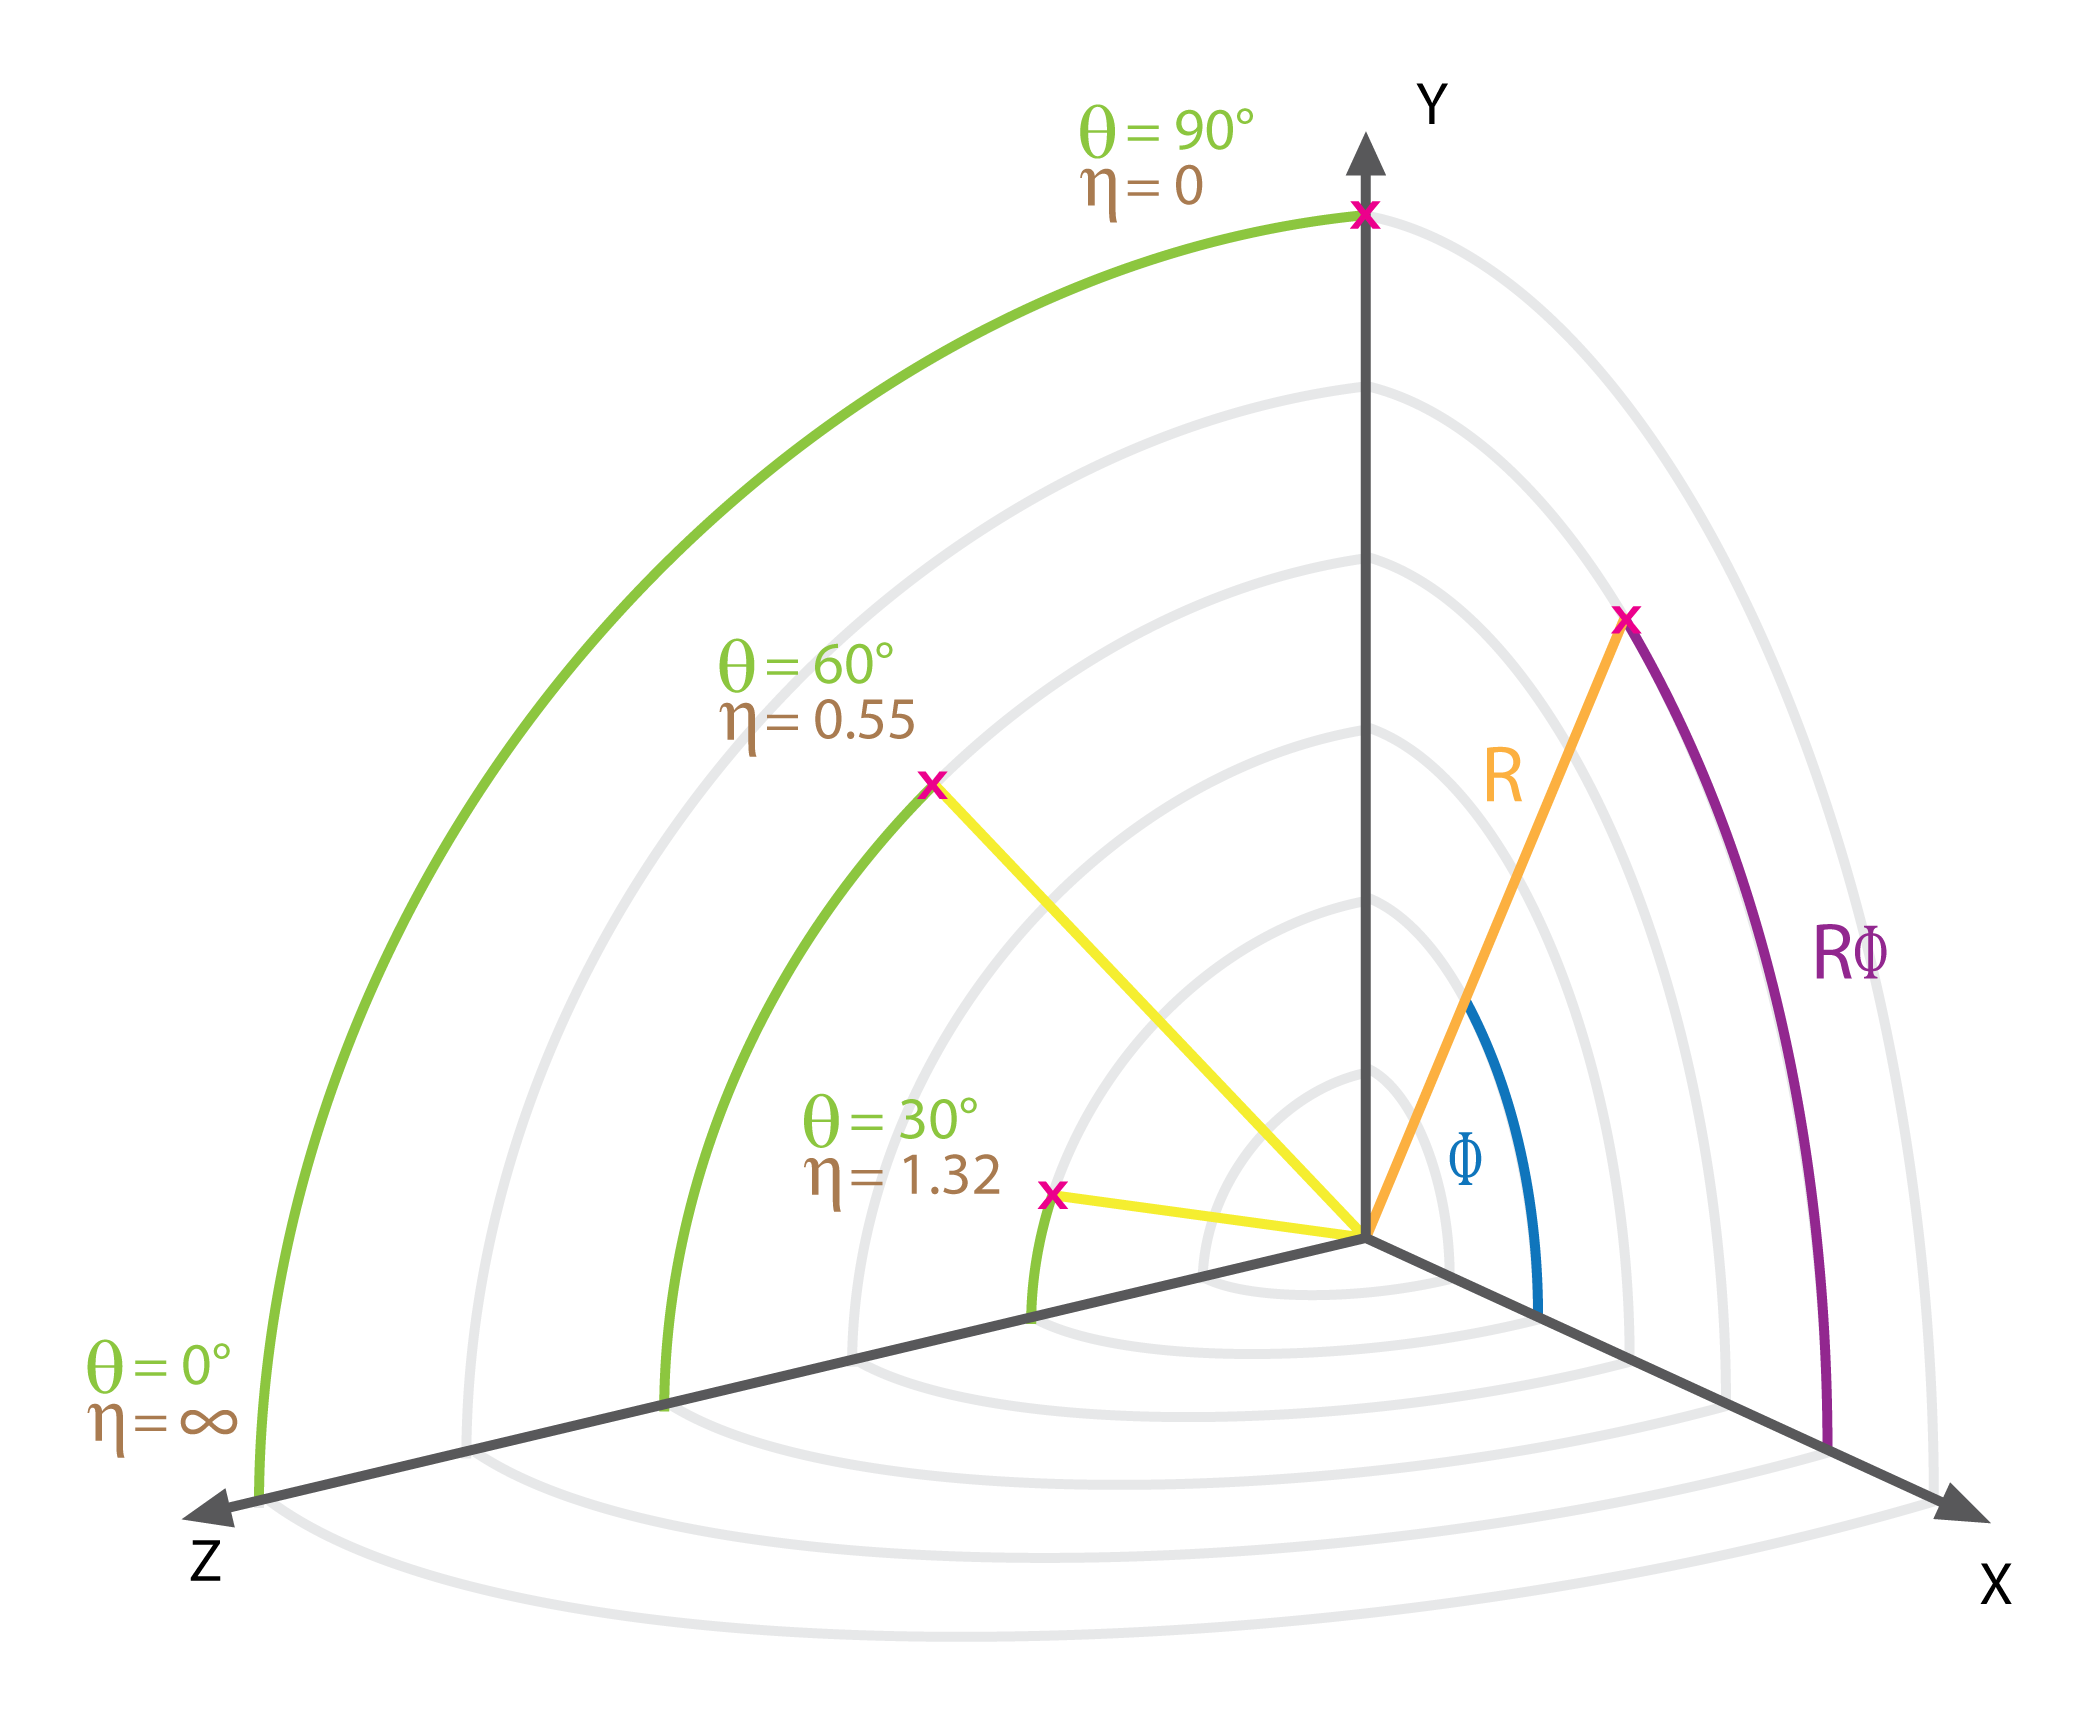
\includegraphics[width=0.6\textwidth]{fig/chapt3/img_cms_coordinates.png}
\caption{\label{fig:CMS_coordinates} An overview of the CMS experiment coordinate system.}
\end{figure}
The azimuthal angle $\phi$ is measured from x axis in the x-y plane where x-y plane is perpendicular to the beam axis and called transverse plane. The polar angle $\theta$ is measured from the z-axis. Instead of $\theta$, angular position is preferentially expressed in terms of a kinematic quantity called pseudorapidity ($\eta$), defined as:
\begin{equation}
\eta \equiv -ln(tan(\frac{\theta}{2}))
\end{equation}
Adopting the above coordinate system, a particle momentum $p$ has two components, one is transverse to the beam direction denoted by $p_{T}$ and calculated from x and y components. The second component is the longitudinal one, $p_{z}$, pointing along the z-axis. Missing transverse energy $E_{T}^{miss}$ term is used for imbalance in total transverse energy of a collision. The angular separation between two particles is usually expressed in $\phi-\eta$ plane expressed as:
\begin{equation}
\Delta R = \sqrt{\Delta\Phi^{2} + \Delta\eta^{2}}
\end{equation} 
In the following sections, a brief summary of all the subsystems of the CMS experiment is given.

%================================================
\subsection{Tracker}
The tracker is the innermost and closest to the interaction point, sub-detector of CMS, immersed in the homogeneous magnetic field of 3.8 T provided by the solenoid.  It is designed to measure the momentum and charge of charged particles emerging from the interaction point by determining the bending of their trajectories in their passage through the detector layers. Secondary vertices can also be reconstructed, associated to the late decays of particles such as B hadrons. The trajectory deviation from the straight line propagation is measured by the sagitta:
\begin{equation}
s \approx \frac{0.3BL^{2}}{8p_{T}}
\end{equation}
Where s is sagitta, B is the solenoid magnetic field, L is the track length and $p_{T}$ is the transverse momentum. The transverse momentum resolution is mainly dependent on the geometric accuracy on the sagitta ($\sigma_{s}$), through:
\begin{equation}
 \frac{\sigma_{p_{T}}}{p_{T}} \approx \frac{8p_{T}}{0.3BL^{2}}.\sigma_{s}
\end{equation}
At the LHC design luminosity and energy (around 1 MHz/mm$^{2}$ at 4 cm from the beamline), several hundreds of particles go through the tracker during each bunch crossing, high granularity, fast response and high radiation tolerance are especially important to its design. To fulfil the aforementioned criteria, the semiconductor silicon technology was chosen to build inner tracking system \cite{tracker}. Charged particles traversing a sensor produce electron-hole pairs which drift under an applied electric field, giving rise to a current pulse. Cooling is ensured by liquid perfluorohexane, maintaining the sensor temperature at around \SI{-10}{\celsius} to limit noise due to radiation-induced leakage\\ 
The tracker occupies a cylindrical volume of 5.8 m in length and 2.5 m in diameter with a surface area of 210 m$^{2}$, extends in the region of $\abs{\eta}$ < 2.5, r < 120 cm, $\abs{z}$ < 270 cm. A schematic view of the CMS tracker is shown in Fig.\ref{fig:tracker}. 

\begin{figure}[h!]
\centering
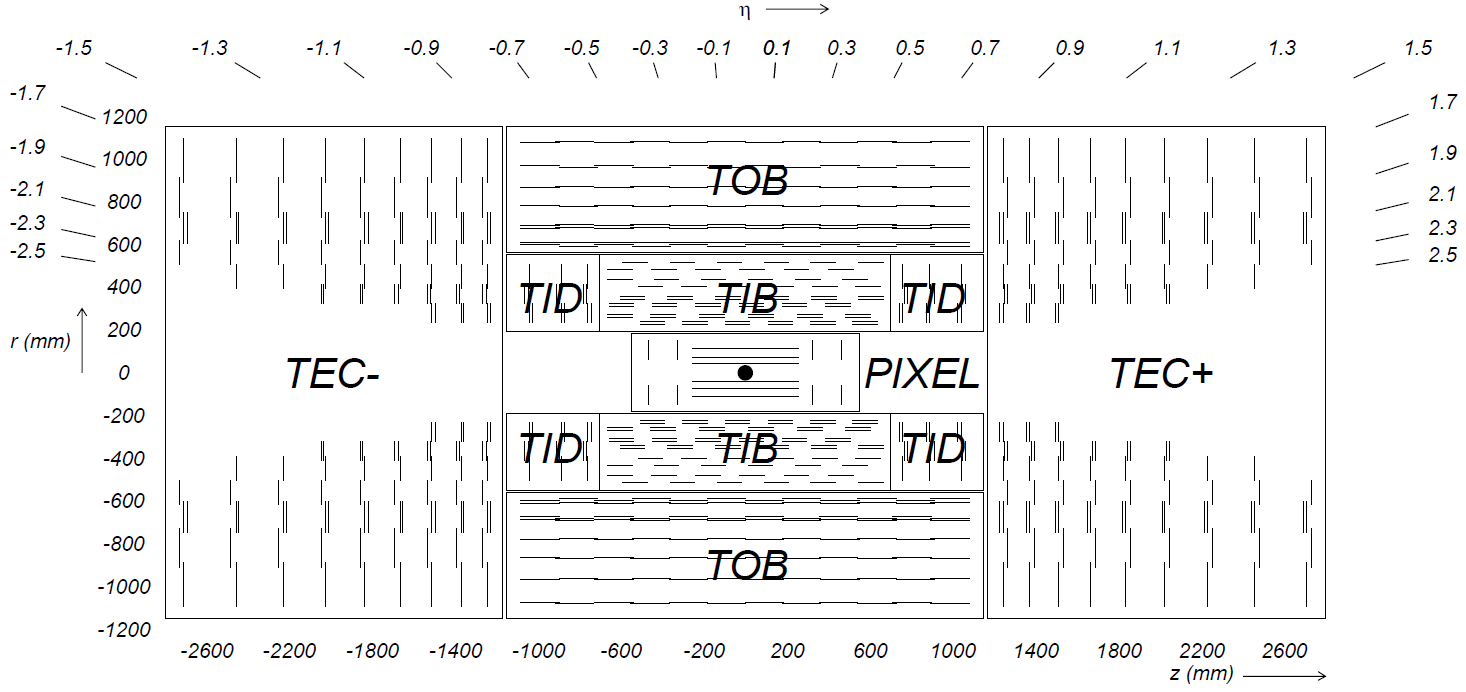
\includegraphics[scale=0.3]{fig/chapt3/Tracker.png}
\caption{\label{fig:tracker} The CMS tracker system with its subsystems in (r, z) plane.}
\end{figure}
The tracker has two sensors classes,  pixel and strip detectors.
\begin{itemize}
\item{\textbf{Pixel Tracker System:}} is placed closest to the interaction point (r $\leq$ 10cm), because of the largest track density. It comprised of a total of approximately 66 million pixel cells grouped in 1440 modules with a cell size of 100 $\times$ 150 $\mu$m$^{2}$. They are arranged in three cylindrical barrel layers at radii between 4.4cm and 10.2cm from the beam line and two endcap discs at each side of the barrel approximately 34.5cm and 46.5cm from the interaction point. With a high reconstruction hit efficiency well above 99\%, the pixel detector covers a pseudorapidity range $\abs{\eta}$ < 2.5, corresponding to the acceptance of the entire tracker. The typical spatial hit resolution is measured to be about 10$\mu$m in the $r-\phi$ plane and 15$\mu$m along the z-axis, while the third coordinate is given by the sensor plane position, allowing for a three-dimensional vertex reconstruction.
\item{\textbf{Strip Tracker System:}} occupies the outer part of the tracker cope with reduced particle density. The silicon strip detector is made of two concentric sets of layers in the barrel (TIB and TOB) occupying the region 20cm < $\abs{r}$ < 55cm and $\abs{z}$ < 118cm and two blocks of forward disks in the endcaps, called TEC and TID covering the region with 55cm < $\abs{r}$ < 116cm and $\abs{z}$ < 118cm.  The single-point resolution is of about 30$\mu$m in the $r-\phi$ plane and 300$\mu$m in the z direction.
\end{itemize} 

%================================================
\subsection{Electromagnetic Calorimeter (ECAL)}
The CMS Electromagnetic CALorimeter (ECAL) \cite{ecal} is an hermetic, homogeneous and high-granularity system made of inorganic scintillating crystals. It's primary aim is to measure precisely position and energy of electrons and photons, which induce electromagnetic showers in the material. The physics process that driven the design of the ECAL is the low mass Higgs decay into two photons $H \rightarrow \gamma\gamma$, one of the leading channels for the study of the Higgs properties. It's role in the $H \rightarrow ZZ \rightarrow 4l$ channel is also important in reconstructing electron together with tracker. ECAL technology is based on lead tungstate (PbWO$_{4}$) scintillating crystals, which act both as absorbers with a short radiation length (X$_{0}$ = 0.89cm) and as scintillators with a very fast response (80\% of the light is emitted within 25ns) which cope with the LHC bunch spacing. Avalanche photodiodes (APD) is used in the barrel and vacuum phototriodes (VPT) in the endcaps to detect the scintillation light with wavelengths around 420nm. An overview of the CMS ECAL is shown in Fig.\ref{fig:ecal}.
\begin{figure}[h]
\centering
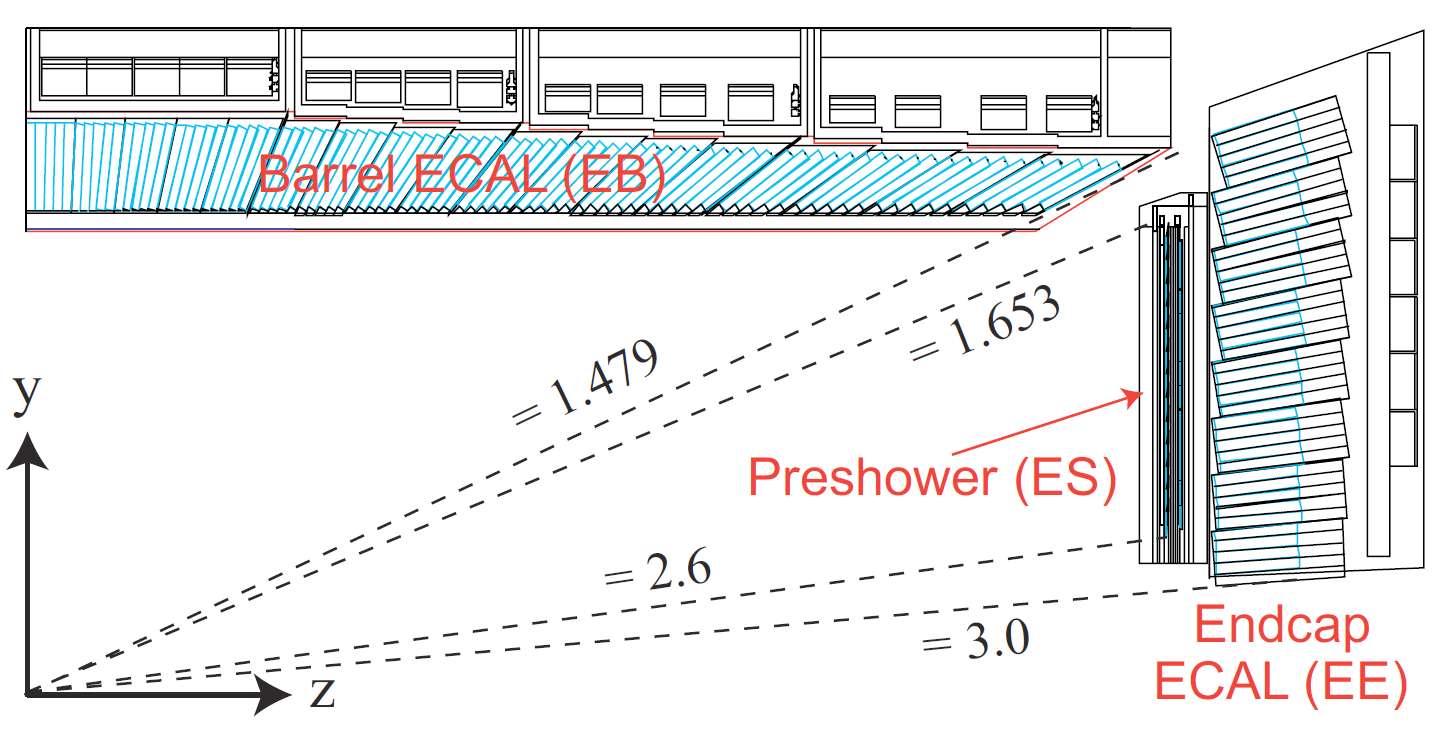
\includegraphics[scale=0.3]{fig/chapt3/img_ECALRapidity.png}
\caption{\label{fig:ecal} The ECAL longitudinal overview of a quadrant.}
\end{figure}
\begin{itemize}
\item{\textbf{ECAL Barrel (EB):}} is located at a distance r = 129cm from the beam axis and it covers the pseudorapidity range 0 < $\abs{\eta}$ < 1.48. It is equipped with 61,200 crystals with a high granularity of 0.0174 $\times$ 0.0174 rad in $\eta-\phi$, each with a transverse section of 22 $\times$ 22 mm$^{2}$ at the front face and a length of 230mm (25.8X$_{0}$). Crystals are grouped in arrays of 2 $\times$ 5, contained in a very thin 200$\mu$m alveolar structure, each corresponding to a sub-module. A group of 40/50 sub-modules are further assembled in modules, where four modules make a super-module.  Finally, EB is divided into 36 super-modules, each subtending an angle of \SI{20}{\celsius} in $\phi$. 
\item{\textbf{ECAL Endcaps (EE):}} is located at a distance $\abs{z}$ = 315.4cm from the interaction point and it covers the range 1.479 < $\abs{\eta}$ < 3 with identically shaped crystals, grouped in carbon-fiber structure of 5 $\times$ 5 elements, called super-crystals. The crystals have a rear face cross section of 30 $\times$ 30 mm$^{2}$, a front face cross section of 28.62 $\times$ 28.62 mm$^{2}$ and a length 220mm (24.7X$_{0}$). Each EE has 134 identical supercrystals with a further 18 sectioned supercrystals to complete the inner and outer perimeter.
\item{\textbf{ECAL Preshawer (ES):}} detectors are placed at each end of the tracker, in front of the EE and cover the pseudorapidity range 1.653 < $\abs{\eta}$ < 2.6. It is a two-layer sampling calorimeter consisting of lead radiator layer with a total of 3X$_{0}$ that initiates electromagnetic showers from incoming particles, and silicon strip sensors that measure the deposited energy and transverse shower profiles. The ES help distinguish $H \rightarrow \gamma\gamma$ decays from single photons, and to identify electrons against minimum ionizing particles.
\end{itemize}
The ECAL energy resolution $\sigma$(E) (for energies below 500 GeV) is given as:
\begin{equation}
(\frac{\sigma_{E}}{E})^{2} = (\frac{S}{\sqrt{E}})^{2} + (\frac{N}{E})^{2} + C^{2}
\end{equation}
where S is the stochastic term due to fluctuations in the lateral shower containment, photostatistics and preshower energy deposition, the second term quantifies the effect of electronic noise and pileup and the constant term is related to the non-uniformity of the longitudinal light collection, calibration uncertainties and energy leakage from the back. The performance of the ECAL barrel module has been studied based on measurements with test-beam data, the typical values of these three parameters obtained are S = 2.8\%, N = 12\% and C = 0.30\% \cite{ecal_resol};

\subsection{Hadronic Calorimeter}
The CMS hadronic calorimeter (HCAL) \cite{hcal} is a hermetic sampling calorimeter, measures precisely the energy and position of charged and neutral hadrons in the form of jets. It also provides an indirect measurement to non-interacting particles in terms of missing energy ($E_{T}^{miss}$). HCAL surrounds the ECAL and the design is restricted by the geometrical dimensions of the ECAL
and magnet systems. A schematic overview of the HCAL is shown in Fig.\ref{fig:hcal} with its four sub-detectors.
\begin{figure}[h!]
\centering
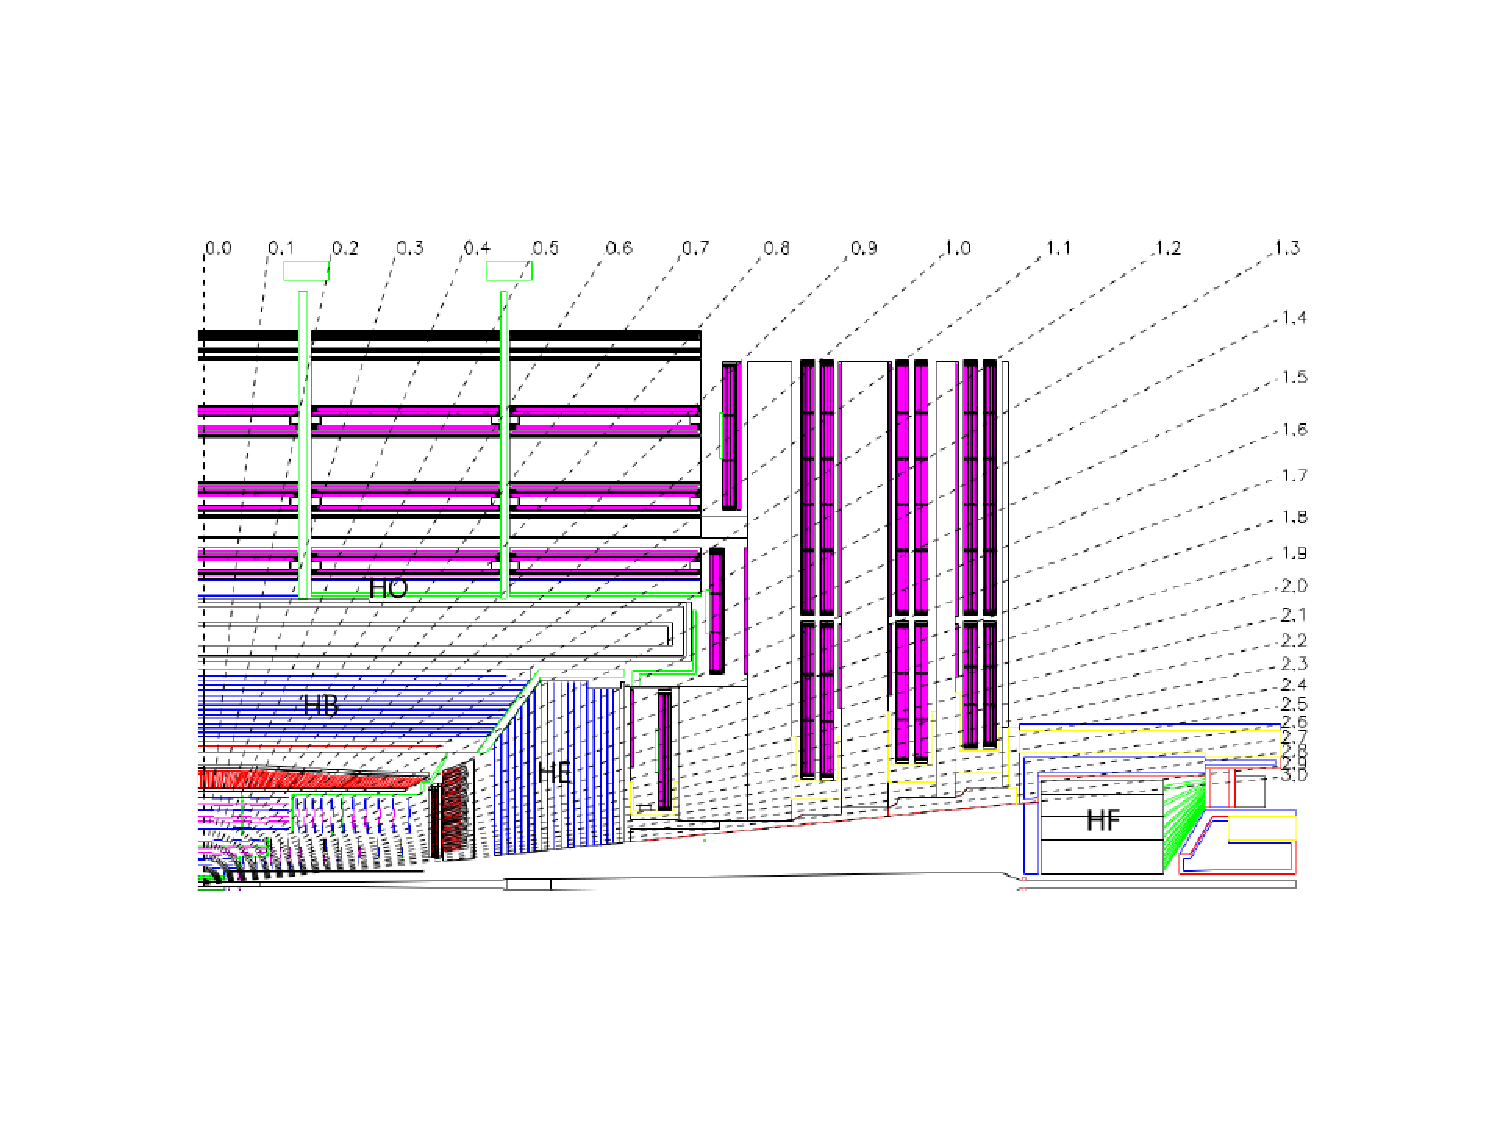
\includegraphics[scale=0.8, trim=90 100 80 80,clip]{fig/chapt3/HCAL.pdf}
\caption{\label{fig:hcal} Longitudinal overview of the one quadrant of the CMS HCAL.}
\end{figure}
The HCAL Barrel (HB) comprise of two half-barrel sections covering a total pseudorapidity range of $\abs{\eta}$ < 1.3, located between EB with r = 1.77m and the inner extent of the magnet coil (r = 2.95m), corresponds to interaction lengths of 5.82$\Lambda_{I}$ in the central region. Due to space restriction, the HB is complemented by an additional layer of scintillators outside the solenoid, referred to as the hadronic outer (HO) calorimeter. HO provides additional depth up to a minimum 11.8$\Lambda_{I}$ to the HCAL system in the radial direction and have same characteristics as HB. \\
The HCAL Endcap (HE) covers forward region in pseudorapidity range of 1.3 < $\abs{\eta}$ < 3.0 and has sufficient depth around 10$\Lambda_{I}$. HB and HE use non-magnetic brass layers as absorber material, and are interspersed with plastic scintillator tiles which serve as the active medium. Two forward hadron calorimeters (HF) are installed which cover the very forward region in pseudorapidity given by 3.0 < $\abs{\eta}$ < 5.0, positioned at $\abs{z}$ = 11.2m from the interaction point, thus ensuring good hermeticity. HF detectors using steel as absorber and Cherenkov-light-emitting quartz fibres are as active medium, motivated by the high particle flux in this region.  The energy resolution of the HCAL system can be expressed in stochastic term a and constant term b as:
\begin{equation}
(\frac{\sigma_{E}}{E})^{2} = (\frac{a}{\sqrt{E}})^{2} + b^{2}
\end{equation}
%=========================================================
\subsection{Magnet}
The CMS detector uses solenoid magnetic field which is the core part of the detector and giving name to the detector. A strong magnetic field is needed to achieve good resolution of the high momentum charged particle upto 1TeV by measuring curvature while direction gives charge of particle \cite{cms_magnet}. The structure of superconducting magnet for CMS  has 6m diameter and 12.5m length, able to generate a uniform magnetic field of 3.8T with a stored energy of 2.3 GJ at full current of 19500A. A graphical overview of the CMS magnetic field is shown in Fig.\ref{fig:magnet}. The magnet mainly uses a superconducting coil (ensured by a helium cooling system at temperature 4K), a vacuum tank (responsible to isolate it from the external environment) and the 10000 ton magnet yoke comprising 5 wheels and 2 endcaps (necessary to return magnetic flux, which otherwise would get lost, disturbing the surrounding environment). 
\begin{figure}[h]
\centering
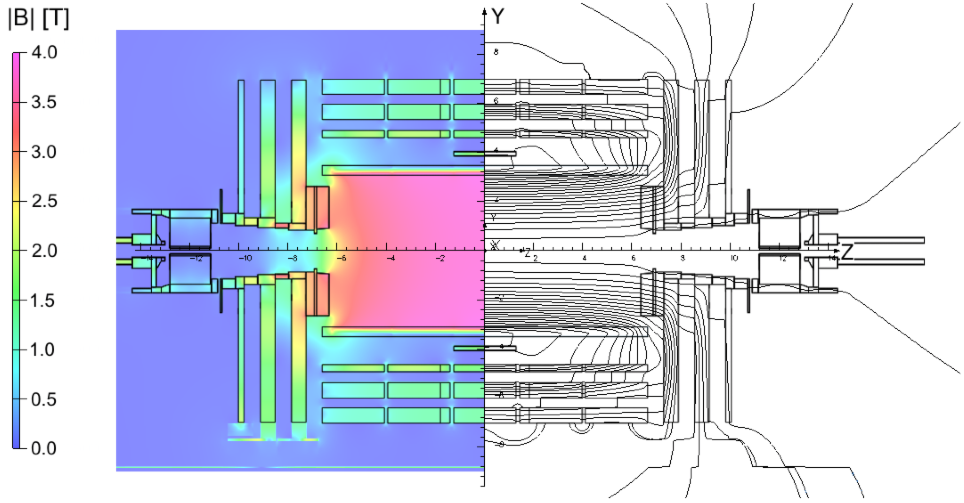
\includegraphics[scale=0.4]{fig/chapt3/Sections_IntroductionFigs_MagField.png}
\caption{\label{fig:magnet} Longitudinal view of the CMS detector magnet where left side shows simulation of the magnetic field and the magnetic field lines are at the right side. At the heart of the detector, the magnetic field value is 3.8T.}
\end{figure}
%========================================
\subsection{Muon Spectrometer}
Muon plays a key role in search for many physics phenomena, ranging from precise measurement of the SM of particle physics to new searches, especially in the discovery of the SM higgs boson through golden channel ($H\rightarrow ZZ \rightarrow 4l$). Being a massive particle compared to electron, muon is less effected by Bremsstrahlung radiations and travel through all the detector subsystems. Using this characteristics, the muon system in the outer region of the CMS detector is embedded in the return yoke of the solenoid. Muons bring a very clean signature to its spectrometer because other particles are stopped by the calorimeters. The CMS muon spectrometer covers a pseudorapidity range to $\abs{\eta}$ < 2.4, consists of three subsystems, Drift Tubes (DTs), Cathode Strips Chambers (CSCs) and Resistive Plate Chambers (RPCs) \cite{cms_muon} as shown in Fig.\ref{fig:rpc_dt}.   

\begin{itemize}
\item{\textbf{Drift Tubes:}}
In the barrel region of the CMS muon system where the magnetic field is mostly uniform and the muon rate is low, four layers of muon stations are installed consists of drift tube (DTs) chambers, covers the pseudorapidity region $\abs{\eta}$ < 1.2. In each wheel, DTs are installed into 12 $\phi$-segments, forming 4 stations in radial direction and interleaved between plates of the magnet flux return yoke. In the longitudinal (except MB4) and bending plane, each station consists of 4 and 8 layers of DTs respectively, to measure precisely the position.\\
DTs consists of an individual cell with grounded walls, acting as cathode and a 50$\mu$m diameter gold-plated stainless-steel anode wire at the center of the cell. The drift electric field is created by two electrode plates mounted at the two sides of the cell. The cells use a gas mixture of 85\% of Ar and 15\% CO$_{2}$ with HV settings: V$_{wire}$ = +3600V, V$_{cath}$ = -1800V and V$_{strip}$ = +1800V \cite{muon-sys}.  
\item{\textbf{Cathode Strip Chambers:}}
Cathode Strip Chambers (CSCs) are installed in the endcap regions with pseudorapidity coverage 0.9 < $\abs{\eta}$ < 2.4. The muon rate and background radiations are higher at the endcaps combine with non-uniform magnetic field, motivated the CSCs to have a fast time response, radiation tolerance and finely segmented. The CSCs operate as standard multi-wire proportional counters, comprise of six planes of anode wires interleaved among seven cathode strips. The anode wires run azimuthally and identify the radial component of a track hit. The cathode strips are oriented radially, almost perpendicular to the wires and provide a precision measurement in the r-$\phi$ bending plane. The CSCs system uses a nominal gas mixture of 40\% Ar, 50\% CO$_{2}$ and 10\% CF$_{4}$.

\item{\textbf{Resistive Plate Chambers:}}
The CMS muon system comprises of a third type of muon detectors, Resistive Plate Chambers (RPCs), installed both in the barrel and endcap regions along with DTs and CSCs, covers the full pseudorapidity range $\abs{\eta}$ < 1.6. RPCs are gaseous parallel-plate detectors, operating in avalanche mode and capable of tagging the time of an ionizing event in times less than 25ns (the bunch crossing time at the design luminosity of the LHC). It makes RPCs an ideal trigger system that provides correct bunch crossing time information between two successive bunches with muons, even at the largest LHC luminosities.
The basic module of the CMS RPC consists of a double-gap chamber where each gap separates two parallel plates of bakelite with a bulk resistivity of 10$^{10}$ - 10$^{11}\Omega$cm. A gas mixture of 95.2\% C$_{2}$H$_{2}$F$_{4}$, 4.5\% i-C$_{4}$H$_{10}$ and 0.3\% HF$_{6}$ using in RPC operation where C$_{2}$H$_{2}$F$_{4}$ is ionized by incident particles and the other two gases prevents the detector from streamer mode. The RPCs operational voltage is lower than 10kV with efficiency about 100\%. Two gases used in RPCs named C$_{2}$H$_{2}$F$_{4}$ and HF$_{6}$ are not environmental friendly that should be replaced by other gases. To cover the full pseudorapidity $\abs{\eta}$ < 2.4 in the endcap region, the present design of the RPC is not suitable to face high flux of particles at the design luminosity of the LHC. A dedicated study is ongoing in the GIF++ facility which summarized in chapter \ref{chapt:10}  
\end{itemize}
\begin{figure}[h]
\centering
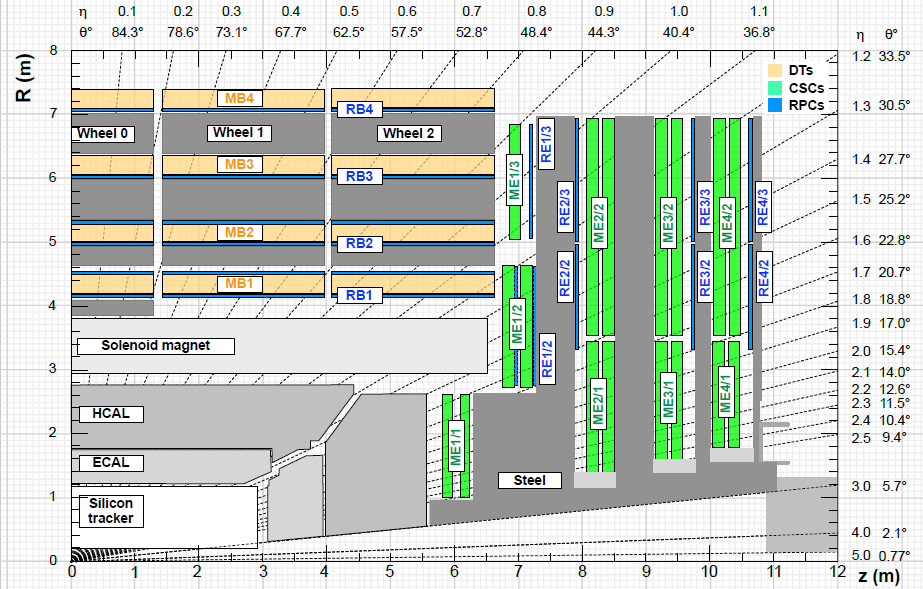
\includegraphics[scale=0.63]{fig/chapt3/muon_detectors.png}
\caption{\label{fig:rpc_dt} The CMS muon system in (R,z) cross section in a quadrant. z is coaxial with beam axis while R is perpendicular pointing upward. DTs are shown by light orange, CSTs by green and RPCs by blue color.}
\end{figure}

%==============================
\subsection{Trigger and Data Acquisition Systems}
The design bunch crossing time of the LHC is 25ns that corresponds to 40MHz frequency and have an average of 20 p-p collision per bunch crossing. This produces an enormous amount of data with 1MB size per event. Due to limitations of detector performance and storage system, the event rate needs a filter to suppress the rate to few hundreds of events per second. CMS uses a dedicated two level (level-1 and level-1) trigger system to control the event rate \cite{cms_trigger}.\\
\textbf{L1 Trigger}: the hardware based trigger system that reduces the rate to 100kHz with a maximum decision time of 4$\mu$s per event. Because of the short decision time, it only uses the calorimeter and muon system information with no tracker information. Local triggers reconstruct primitives particles candidates in each component of a given subdetector which are combined by regional triggers to construct higher level L1 objects (muons, electrons and jets) and subsequently merged into global trigger which decides to select or reject the event. \\
\textbf{HLT}: After the L1 trigger, event rate is further reduced to 40Hz by using high level trigger (HLT), a software based trigger that uses information from all subsystems. The reconstruction and selection used by HLT software is similar to the offline reconstruction and selection which takes place in two successive stages follow the basic principle of time minimization for each event. In first stage (Level-2), HLT takes input from L1 and reconstructs the basic objects from calorimeters and muon system. In second step (Level-3) of the HLT, the full information from the tracker is accessed for track reconstruction and vertices. The event is finally selected and permanently stored for offline analysis if the requirements of at least one HLT path are met.

  



\clearpage{\pagestyle{empty}\cleardoublepage}
